\chapter{Tree Variational Autoencoder}\label{ch:tree2tree}
\begin{remark}
    An earlier revision of this chapter \cite{liventsevTreeVariationalAutoencoder2025} has been published at IEEE Access
\end{remark}

\section{Motivation}

In chapters \ref{ch:bfpp} and \ref{ch:neurogen} we used \text{BF++}, a \emph{domain-specific language} (section \ref{sec:dsl}) to prevent the optimization space from growing unmanageably sparse (as discussed in section \ref{sec:ps-challenge}).
Extending these techniques to work with an arbitrarily complex programming language would offer numerous benefits in terms of expressivity and compatibility with the rest of the software ecosystem.

Can we combine the simplicity of neurogenetic optimization in \emph{BF++} space with the advantages of a popular language \cite{tiobe2017tiobe}?
One approach would be to train a foundational (section \ref{sec:pretrain}) autoencoder \cite{autoencoders} model for code.
Such a model can be trained in an unsupervised fashion on a corpus of code and be used to represent a complex program as a vector in a latent space of lower dimensionality.
Then, neural, genetic and/or neurogenetic optimization methods could operate directly on this low-dimensional representation, i.e. a program can be mutated by adding random noise to its embedding vector and several can be merged by averaging their embedding vectors.

Indeed, Autoencoder Genetic Programming has been studied previously \cite{wittenbergDenoisingAutoencoderGenetic2023,latentspaceopt}, though often with underwhelming results \cite{autoenc-gp}.
Following the success of structural models of code (see section \ref{sec:grammar-guided}), we hypothesize that the difficulties facing Autoencoder Genetic Programming can be addressed by harnessing the grammatical structure of code that can be trivially obtained from a compiler, but gets ignored in \cite{wittenbergDenoisingAutoencoderGenetic2023,latentspaceopt,autoenc-gp}.

In this chapter we develop a variational autoencoder for code that operates on programs as abstract syntax trees rather than sequences of tokens to explore \rqtree:

\begin{highlight}
    would a model that operates directly on the program's Abstract Syntax Tree learn a better latent representation of the source code than a model that operates on a sequence of tokens?
\end{highlight}

To the best of our knowledge the advantage of structural models has not been tested in autoencoders for genetic programming. 
\cite{kusner2017grammar,grammar-vae} find that it is beneficial to include grammatical metadata in token representations for a traditional sequence model, but do not employ a tree-based encoder-decoder architechure.

\newpage
\section{Proposed architecture}

The proposed model, \emph{Tree2Tree}, is a variational autoencoder with a Child-sum TreeLSTM as the encoder (section \ref{sec:encoder}) and a Doubly Recurrent Neural Network (section \ref{sec:decoder}) extended with add gate mechanism as the decoder.
Variational autoencoder \cite{kingma2013auto} is chosen since its Kullback-Leibner component encourages the model to use the smallest subspace of the latent space possible, making the model less brittle with respect to the dimensionality of the latent space than its deterministic counterpart.
However, our experiments in section \ref{sec:results} indicate that latent vector size remains important.

\subsection{Encoder}
\label{sec:encoder}
The encoder network aims to capture the most relevant information in a program and map it to a smaller representation. 

\paragraph{Embedding layer} The first layer of the encoder network convert tokens into dense representations, which can be initialized randomly or with pre-trained parameters and then fine-tuned further.


\paragraph{Tree-LSTM} We employ the Child-Sum Tree-LSTM \cite{tai2015improved} which is defined as follows. Given some tree, we use $\treenode$ to denote a node, $\mlinputvec^\treenode$ to denote its vector representation, $\treenode(\treenode')$ to state that $\treenode$ is a parent of $\treenode'$ and $\treenode < \treenode'$ to state that $\treenode$ is to the left of $\treenode'$ because the part of the program $\treenode$ represents occurred before the part of the program represented by $\treenode'$.
Given these inputs, Child-Sum Tree-LSTM computes a hidden state $\hidden^\treenode$ for every node of the tree as follows:

\begin{align}\label{eq:tree_lstm_encoder}
    \hidden^\treenode_{*} &= \sum_{\treenode' \in C(\treenode)} \hidden^{\treenode'} \\
    \hidden_i^\treenode &= \stddev(\weights^\mlinputvec_{i} \cdot \mathbf{x}^\treenode + \weights^\hidden_{i} \cdot \hidden^\treenode_* + \biases_{i})  \\ 
    \hidden_f^{\treenode \treenode'} &= \stddev(\weights^\mlinputvec_{f} \cdot \mathbf{x}^\treenode + \weights^\hidden_{f} \cdot \hidden^{\treenode'} + \biases_{f}) \\\label{eq:child_sum_4}
    \hidden_o^\treenode &= \stddev(\weights^\mlinputvec_{o} \cdot \mathbf{x}^\treenode + \weights^\hidden_{o} \cdot \hidden^\treenode_* + \biases_{o}) \\
    \hidden_u^\treenode &= tanh(\weights^\mlinputvec_{u} \cdot \mathbf{x}^\treenode + \weights^\hidden_{u} \cdot \hidden^\treenode_* + \biases_{u}) \\
    \hidden_c^\treenode &= \hidden_i^\treenode \odot \hidden_u^\treenode + \sum_{\treenode' \in C(\treenode)} \hidden_f^{\treenode \treenode'} \odot \hidden_c^{\treenode'} \\
    \hidden^\treenode &= \hidden_o^\treenode \odot tanh(\hidden_c^\treenode)
\end{align}

In eq. \ref{eq:child_sum_4}, $\treenode'(\treenode)$ and $\odot$ denotes the element-wise product (Hadamard product), whereas $\stddev$ and $\tanh$ refer to elementwise sigmoid and hyperbolic tangent. 
\begin{equation}
    \weights^\mlinputvec, \weights^\hidden, \biases \in \learnables
\end{equation}
where $\learnables$ are trainable parameters of the model. 
Note that node $\treenode$ depends on the hidden states of its children. 
In other words, Tree-LSTM is computed bottom-up. 

Just like the standard LSTM model, Tree-LSTM can be stacked to create a multilayer Tree-LSTM. 
We use a 3-layer architecture, in which the hidden state of a Tree-LSTM unit in layer $l$ is then used as input to the Tree-LSTM unit in layer $l + 1$ in the same time step, the same as with the standard LSTM \cite{graves2013hybrid}. 
The design intention is to allow higher layers to capture longer-term dependencies of the input, which in the case of Tree-LSTMs translates to capturing longer-term dependencies along the paths of a tree.

\begin{figure}
    \centering
    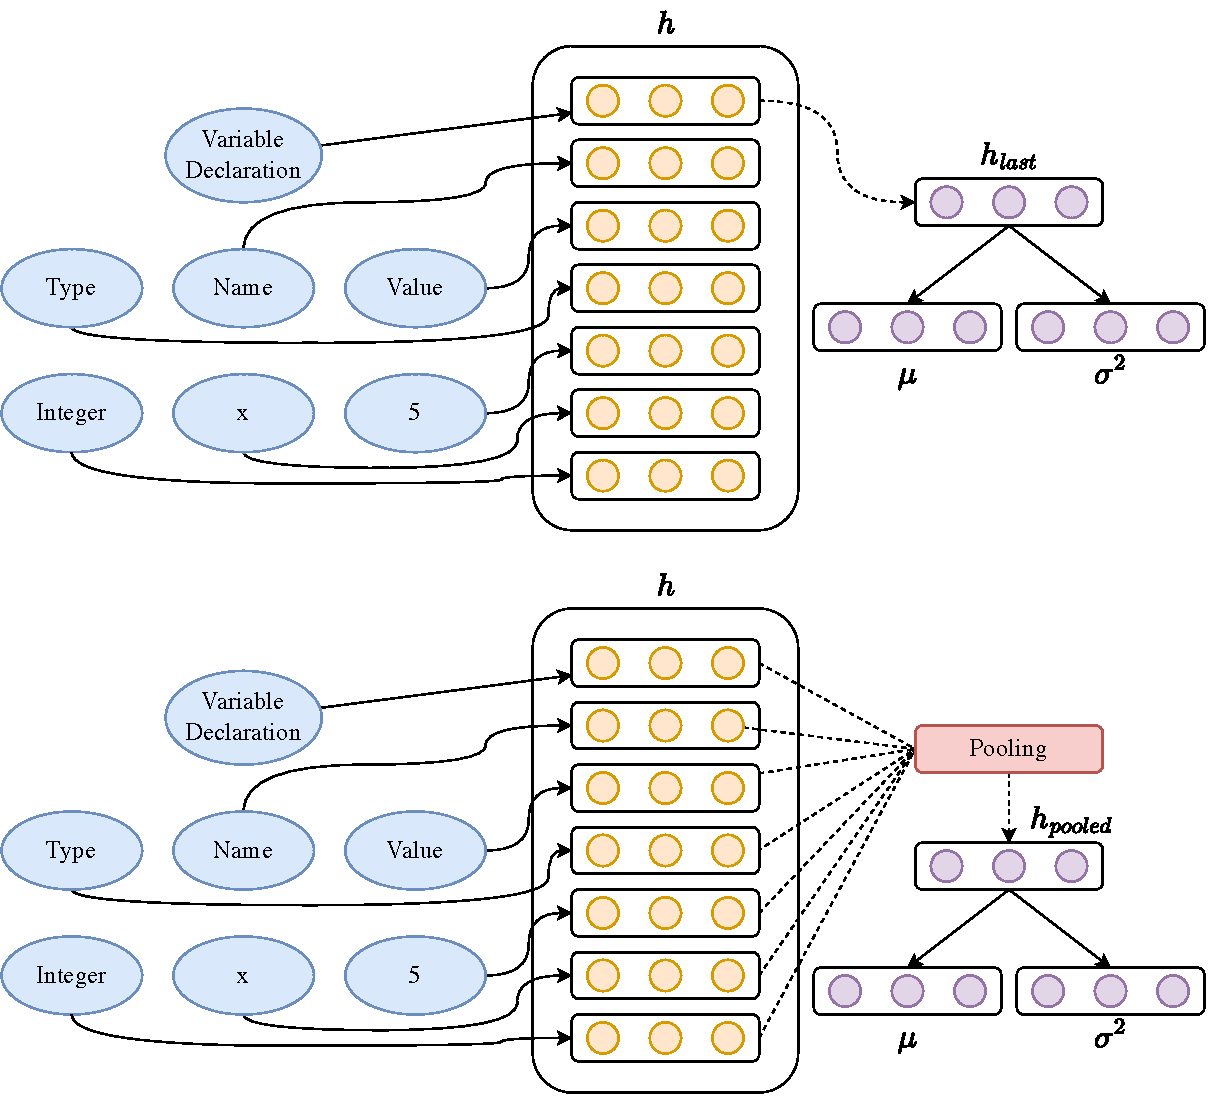
\includegraphics[width=\linewidth]{pooling.pdf}
    \caption[RNN pooling]{\textbf{Top}: Typical architecture of encoder model of VAE in which only the last hidden state from the RNN is used to compute the mean $\mean$ and variance $\stddev^2$. \textbf{Bottom}: A pooling method to aggregate the hidden states from the RNN to compute the mean $\mean$ and variance $\stddev^2$.}
    \label{fig:pooling}
\end{figure}




\paragraph{Neural attention} Tree-LSTM layers are followed by an attention layer. 
The node importance calculation is based on \cite{winata2018attention}, and updates the hidden states as follows:
\begin{align}
    \hidden_{at} = \hidden \odot tanh(\weights^\mlinputvec \cdot \hidden + \biases)
\end{align}

Here, $\hidden$ denotes the hidden states of the last Tree-LSTM layer. This additional layer allows the network to prioritize nodes that contain the most information. 


\paragraph{Pooling} 
The last step in the architecture is the pooling layer responsible for compressing the sequence of $h_{at}$ into a fixed size vector $h_\text{pooled}$. 
We rejected a common \cite{fabius2015variational} approach of only taking the last hidden state of the RNN as the input to the decoder due to the long-term memory loss problem \cite{kao2020comparison} and use max pooling instead.
See figure \ref{fig:pooling} for details.

\paragraph{Sampling latent code} The pooled vector is then used to compute the mean and variance of the approximate posterior to sample a latent code $\latent \sim \normaldistr(\mean, \stddev)$ with the help of the reparametrization trick \cite{kingma2013auto}. The mean and variance are computed using linear layers with learnable weights $\weights_{\mean}$, $\weights_{\stddev}$ and biases $\biases_{\mean}$, $\biases_{\stddev}$:

\begin{align}
\mean& = \weights_{\mean} h_\text{pooled} + \biases_{\mean} \\
\stddev& = \weights_{\stddev} h_\text{pooled} + \biases_{\stddev} \\
\latent & = \mean+ \stddev\odot \boldsymbol{\epsilon}, \quad \boldsymbol{\epsilon} \sim \normaldistr(0, \hidden_i)
\end{align}
\newpage
\subsection{Decoder}
\label{sec:decoder}

\paragraph{Tree decoding} We use the same tree structure for decoding as we used for encoding. 
Having the order of the input sequence reversed compared to the reconstructed sequence has been shown in \cite{fabius2015variational} to improve the performance of the model. 
We employ this technique in our model, which means that since our encoder processes trees bottom-up, the decoder will produce trees top-down. 
The idea here is that the first steps of decoding the tree are more related to the latent space than the last steps.



A method known as Doubly-Recurrent Neural Network (DRNN) \cite{alvarezmelis2017tree} allows for top-down tree generation from an encoded vector representation. This method operates solely on the vector representation and does not require that either the tree structure or the nodes are given. The DRNN is based on two recurrent neural networks, breadth and depth-wise, to model ancestral and fraternal information flow. For some node $\treenode$ with parent $pa(\treenode)$ and previous sibling $s(\treenode)$, the ancestral and fraternal hidden states are computed as follows:

\begin{align}
    \hidden_a^\treenode &= rnn_a(\hidden_a^{pa(\treenode)}, \hidden_i^{pa(\treenode)}) \\ \label{eq:ancestral_update}
    \hidden_f^\treenode &= rnn_f(\hidden_f^{s(\treenode)}, \hidden_i^{s(\treenode)}) 
\end{align}

Where $rnn_a$, $rnn_f$ are functions that apply one step of the ancestral and fraternal RNNs, respectively. Furthermore, $\hidden_i^{pa(\treenode)}$, $\hidden_i^{s(\treenode)}$ are the input values (label vectors) of the parent and previous sibling respectively. After the ancestral and fraternal states of $\treenode$ have been computed with the observed labels of its parent and previous sibling, these states can be combined to form a predictive hidden state:

\begin{align}
    \hidden^\treenode_{pred} = \tanh\left((\weights^\mlinputvec_a \cdot \hidden_a^\treenode + \biases_a) + (\weights^\mlinputvec_f \cdot \hidden_f^\treenode + \biases_f)\right)
\end{align}

Where the operations applied to $\hidden_a^\treenode$, $\hidden_f^\treenode$ are linear layers with learnable weights and biases. This combined state then contains information about the nodes' neighbors in the tree.



For each node in the tree, the model needs to decide whether it has offspring and whether it has any successor siblings. We can use the predictive hidden state of a node $\hidden^\treenode_{pred}$, with a linear layer and a sigmoid activation to compute the probability for offspring and successor siblings as:

\begin{align}
    \prob_a^\treenode &= \stddev(\weights^\mlinputvec_{pa} \cdot \hidden_{pred}^\treenode + \biases_{pa}) \label{eq:prob_ancestral} \\
    \prob_f^\treenode &= \stddev(\weights^\mlinputvec_{pf} \cdot \hidden_{pred}^\treenode + \biases_{pf})\label{eq:prob_fraternal}
\end{align}

During training, we use the actual values for whether a node has children and successor siblings. 
During inference, we can randomly sample from $\prob_a^\treenode,\prob_f^\treenode$ or choose a confidence level to continue creating offspring and succeeding siblings as long as the probability stays above the chosen threshold. 

\paragraph{Constrained decoding}
Applying DRNN \cite{alvarezmelis2017tree} to code entails special advantages: grammatical constraints of the programming language can be used to narrow down the token vocabulary for the model to select from.
We identify 3 Abstract Syntax Tree parent nodes that impose specific constraints onto possible children:

\begin{enumerate}
    \item \textbf{Literal:} the children of this node represent a literal, i.e. a number or a string
    \item \textbf{Type:} the children of this node represent the name of a valid C++ type
    \item \textbf{Built-in function reference:} the child of this node has to be the name of a built-in function
\end{enumerate}

When one of these nodes is encountered during tree decoding, we apply one of the specialized linear layers
\begin{equation}
\langle W_o,b_o \rangle \in \{\langle W_\text{literal},b_\text{literal} \rangle, \langle W_\text{type},b_\text{type} \rangle, \langle W_\text{builtin},b_\text{builtin} \rangle \}
\end{equation}

to predict the value of a child token. Its token probability distribution over the subvocabulary allowed by the parent token is defined as

\begin{align}
    \hidden_o^\treenode =  softmax\left(\weights_o \cdot \hidden_{pred}^\treenode + \biases_{o}\right) \label{eq:label_pred}
\end{align}

For literal tokens, the vocabulary can, in theory, be infinitely large. We employ adaptive softmax \cite{grave2017efficient} to use a vocabulary consisting of many unique literal tokens without a considerable increase in computational complexity.

A leaf node that does not have one of the 3 special parents is either a \textbf{reserved token} (for, if, while, ...) or an \textbf{identifier}. We predict whether it's a reserved token using another linear layer, the same way as the topology predictions using the predictive hidden state of the node: 

\begin{align}
    p_r^\treenode &= \stddev(\weights_{pr} \cdot \hidden_{pred}^\treenode + \biases_{pr}) \label{eq:res_pred}
\end{align}

For reserved tokens, another linear layer $\langle W_o,b_o \rangle = \langle W_\text{reserved},b_\text{reserved} \rangle$ is used to predict the value.

\paragraph{Identifier tokens}
Since program behavior is invariant to identifier replacement, instead of attempting to accurately predict identifier names we map each unique identifier to a reusable ID \cite{tufano2019learning} and treat the prediction of identifiers as a clustering problem. 

The model can keep track of a list of the declared identifiers while generating an AST. Each time a new identifier is declared, a new reusable ID is added to the list. Then for each reference, we can compute the similarity to each of the declared identifiers using some similarity function and predict the most similar identifier. Let $D$ be the set of currently declared identifier nodes and $\treenode$ be the current reference node we are trying to predict, the most similar declared identifier can be computed as follows:

\begin{align}
    \mathbf{s}^{\treenode \treenode'} &= similarity(\weights_c \cdot \hidden^\treenode_{pred} + \biases_c,  \weights_c \cdot \hidden^z_{pred} + \biases_c) \\
    \mathbf{r}^\treenode &= \min_{\treenode' \in D}(\mathbf{s}^{\treenode \treenode'})
\end{align}

\paragraph{Add gate} \label{par:addgate} The DRNN model has a large flaw, where it is not able to differentiate between paths with the same prefix. For example, consider two function declarations named `add' and `main' depicted in the upper part of figure \ref{fig:treeAddGate}. In the original formulation of DRNN \cite{alvarezmelis2017tree} there is no information flow from the left sibling of the parent to the child, resulting in both name nodes having the exact same hidden state and thus the same label. To solve this issue, we would like to incorporate fraternal states in the downwards flow for the model. Hence, we revise equation \ref{eq:ancestral_update}, where we take inspiration from the LSTM model and apply the idea of the add gate to our ancestral update formula:

\begin{align}
    &\hidden_{mf}^\treenode = \stddev(\weights^\mlinputvec_m \cdot \hidden_f^\treenode + \biases_m)\\
    &\hidden_{af}^\treenode = tanh(\weights^\mlinputvec_a \cdot \hidden_f^\treenode + \biases_a)\\
    &\hidden_a^\treenode := \hidden_a^\treenode + (\hidden_{af} * \hidden_{mf})
\end{align}

The formulas above apply an update to the calculated hidden state of the node based on the hidden state of the left sibling of its parent, as depicted in the bottom part of figure \ref{fig:treeAddGate}. The update is gated: $\hidden_a^\treenode$ determines the residual vector (with values in the range of $[-1,1]$) to be added to $\hidden_a^\treenode$, while $\hidden_{mf}^\treenode$ acts as attention mask deciding which parts of the state shall or shall not be updated based on the available information.


\begin{figure}
    \centering
    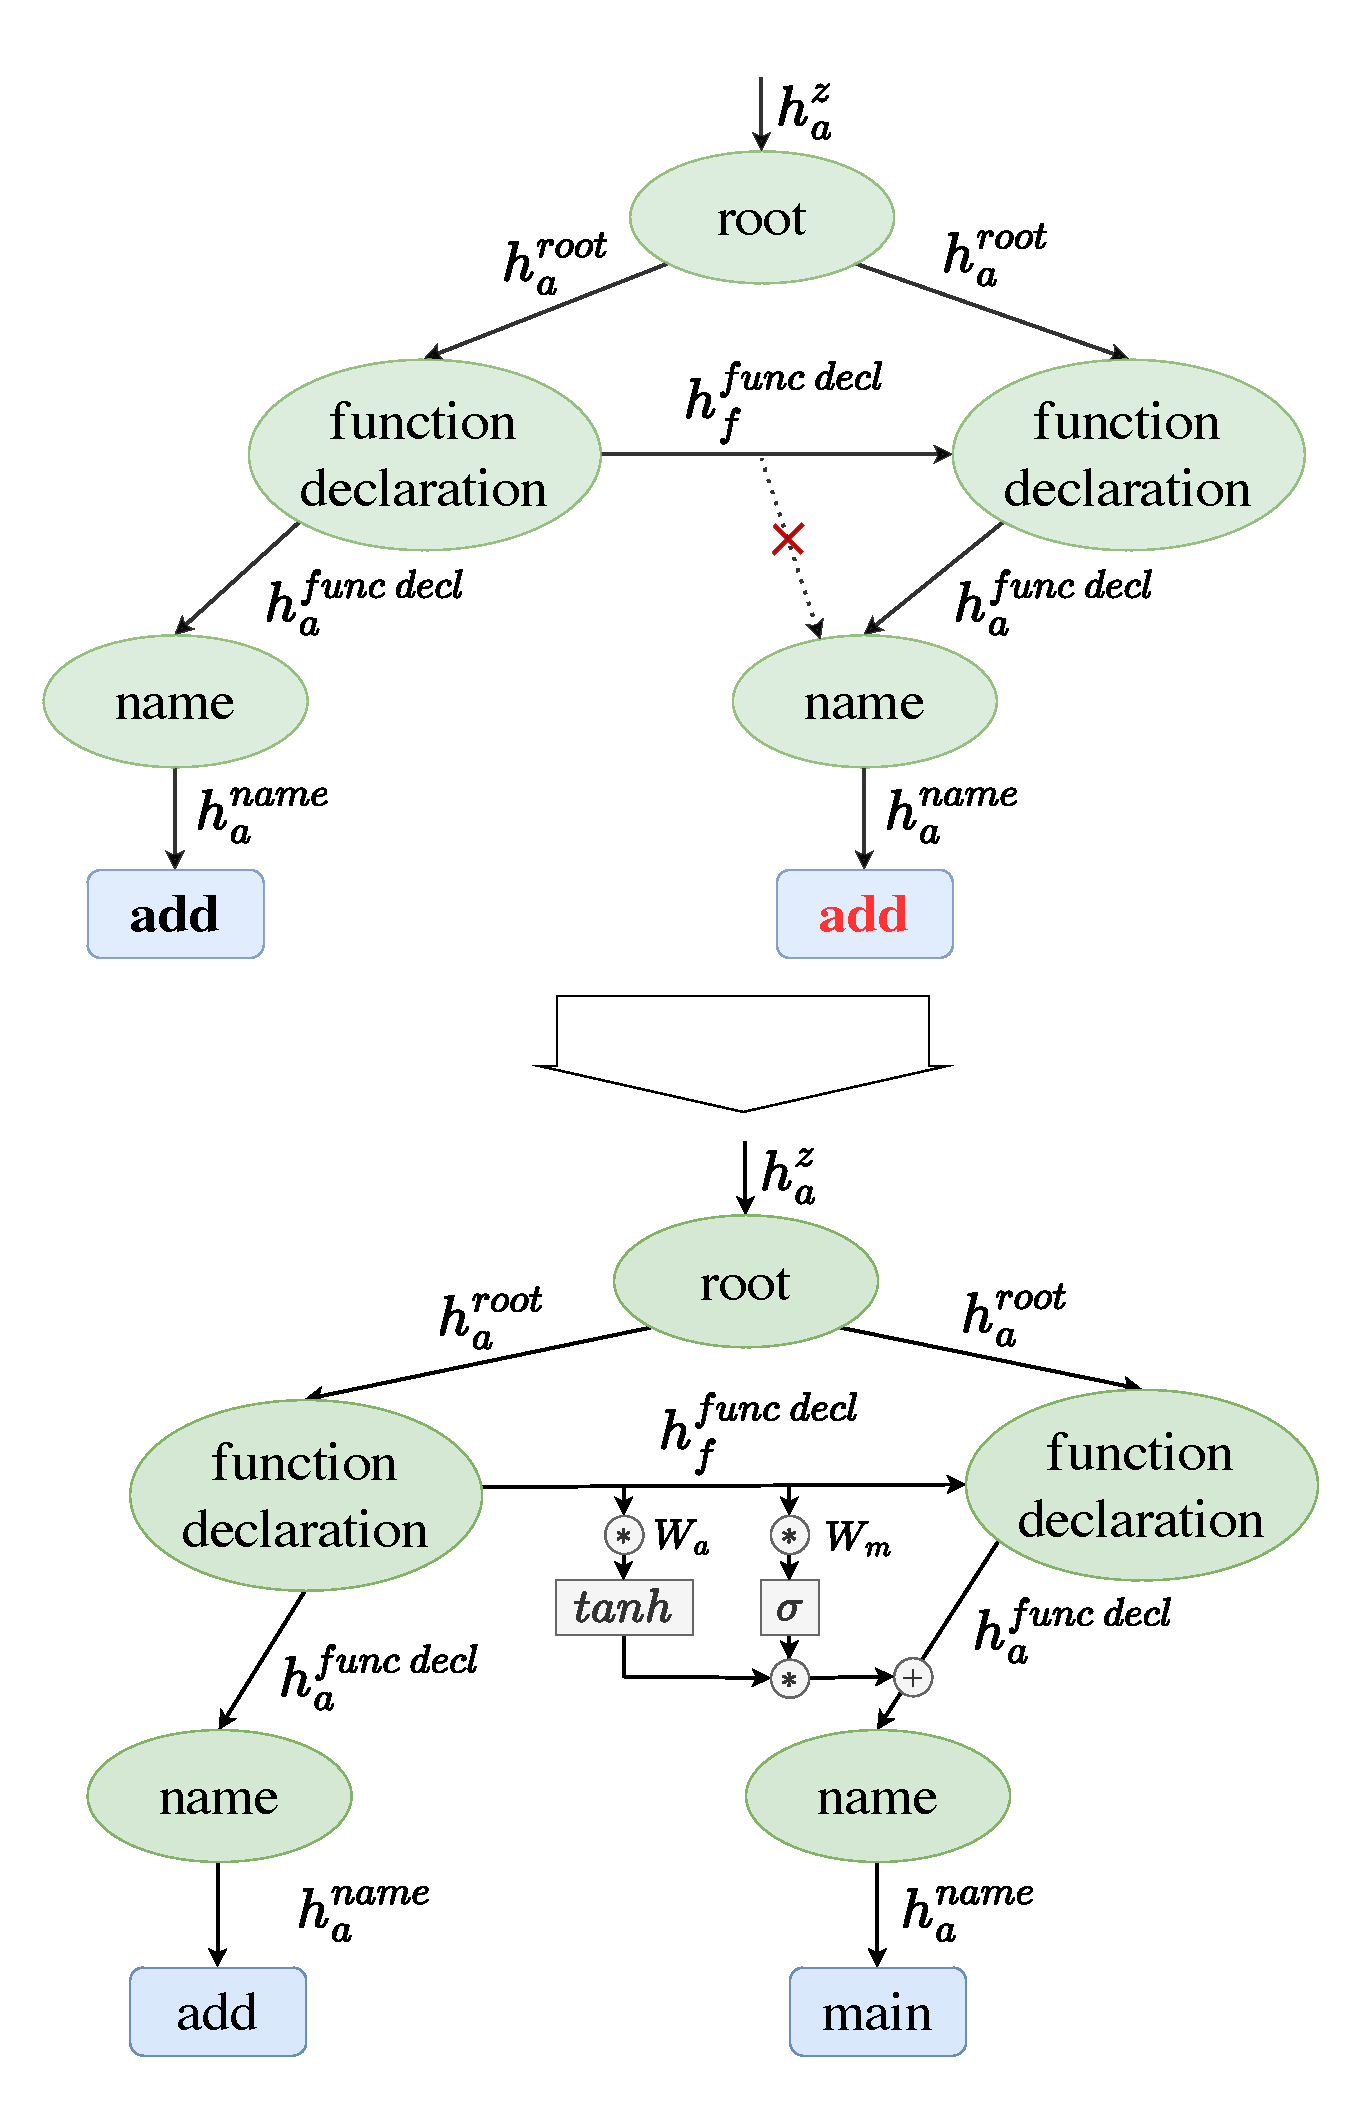
\includegraphics[width=\linewidth]{images/TreeAddGate.pdf}
    \caption{DRNN expanded with an add gate to allow for information flow from previous siblings downwards}
    \label{fig:treeAddGate}
\end{figure}

\newpage
\subsection{Batching}

\begin{figure}
    \centering
    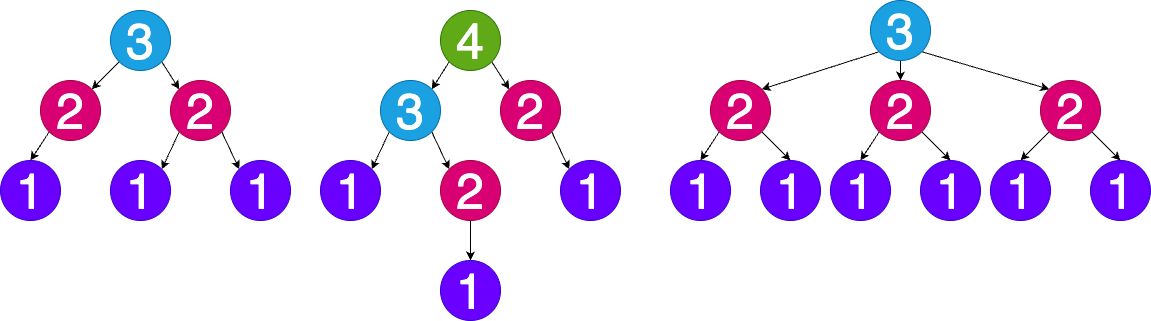
\includegraphics[width=\linewidth]{images/TreeBatchingEncoder.png}
    \caption{Node processing sequence in the encoder.}
    \label{fig:treeBatchingEncoder}
\end{figure}

\begin{figure}
    \centering
    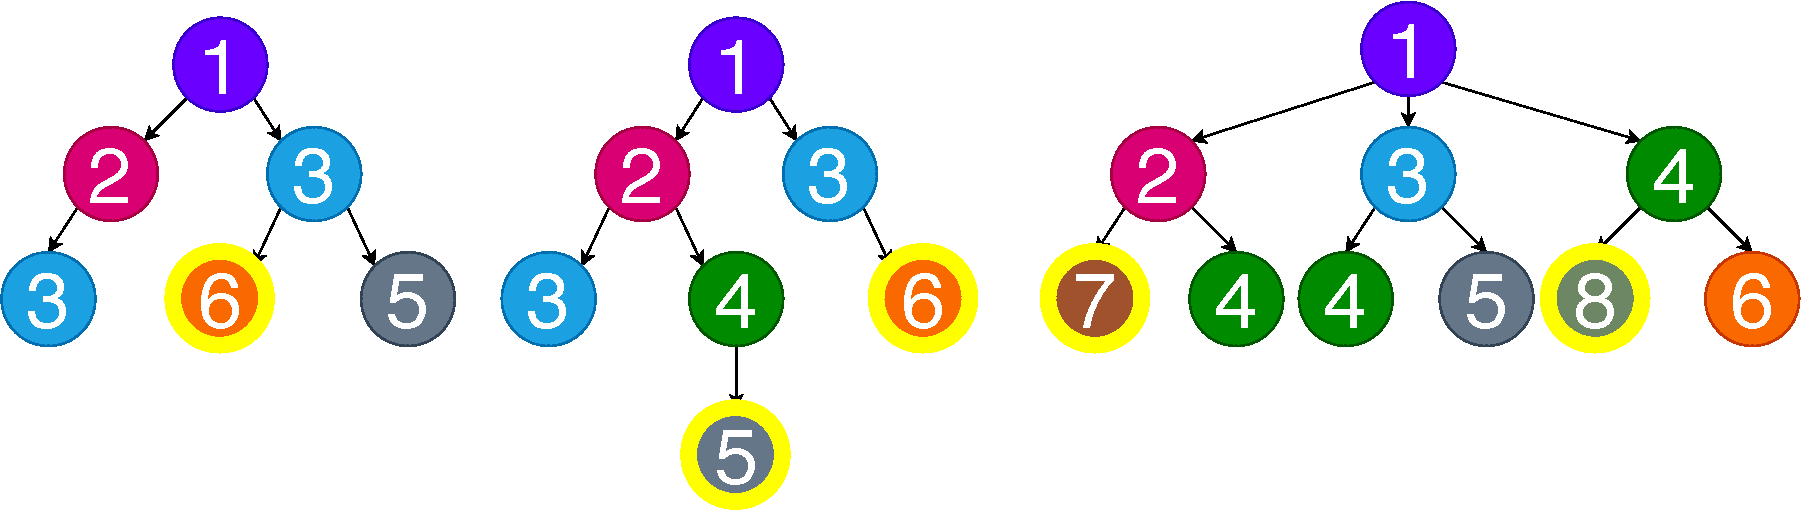
\includegraphics[width=\linewidth]{images/TreeBatchingIdentifiers.pdf}
    \caption{Node processing sequence in the decoder. Yellow outline indicates identifier nodes.}
    \label{fig:treeBatchingDecoder}
\end{figure}

When computing the above equations for all nodes of the tree, many operations are mutually independent and can be processed in parallel.
Following the principles of data flow programming \cite{schwarzkopfRemarkableUtilityDataflow2020}, we can break the computation graph down into batches that can make use of parallel computation capabilities of modern GPUs.
In the first batch, we compute all nodes that don't depend on other nodes in the tree.
In the second batch, we compute all nodes that only depend on nodes from the first batch and so on.

In the encoder this approach results in an intuitive bottom up processing sequence as seen in figure \ref{fig:treeBatchingDecoder}, starting with a batch of all leaves of the tree, followed by their parents, then grandparents and so on until the hidden state of the root is found.
For the decoder, the processing sequence is more complex, since the hidden state of the node depends on both its parent and its left siblings (see equations 18-20), resulting in "diagonal" batches where the children and right-siblings of nodes of batch $i$ are processed in batch $i+1$, starting with batch $1$ that only includes the root.
Our clustering algorithm for resolving identifier tokens (section \ref{sec:decoder}) requires that identifier tokens are processed strictly left to right, to make sure that variable references are processed before respective variable declarations.
This does not always hold under "diagonal" batching, especially if the tree is left-skewed, so we handle identifier tokens exceptionally, from left to right, after all other nodes have been processed.
The middle tree in figure figure \ref{fig:treeBatchingDecoder} is such an example: its 2 identifier tokens would be processed out of order if not for this exception.

\subsection{Optimization}

\paragraph{Mitigating KL vanishing}
KL vanishing is a common issue when dealing with VAEs with a decoder parameterized by an auto-regressive model.
We mitigate it using cyclical KL cost annealing \cite{fu2019cyclical}. 
Furthermore, we apply pooling to the hidden states of the RNN network in the encoder. Long \textit{et al.} \cite{long2019preventing} show this pooling method can effectively prevent posterior collapse. 

\paragraph{Loss function}
We use binary cross-entropy loss for the binary classification problems of predicting whether a node $\treenode$ has offspring

\begin{align}
    \loss_{a}(\treenode) = \begin{cases}
        \log(p^\treenode_a) & \text{if }\exists \treenode' | \treenode(\treenode') \\
        \log(1- p^\treenode_a) & \text{otherwise}
    \end{cases}
\end{align}

successor siblings

\begin{align}
    \loss_{f}(\treenode) = \begin{cases}
        \log(p^\treenode_f) & \text{if }\exists \treenode_p, \treenode_s | \treenode_p(\treenode), \treenode_p(\treenode_s), \treenode_s > \treenode \\
        \log(1- p^\treenode_f) & \text{otherwise}
    \end{cases}
\end{align}

and whether this node belongs to the reserved token category (equation \ref{eq:res_pred})

\begin{align}
    \loss_{r}(\treenode) = \begin{cases}
        \log(p^\treenode_r)  & \treenode \text{ is reserved} \\
        \log(1- p^\treenode_r)  & \text{otherwise}
    \end{cases}
\end{align}

Label prediction is a classification problem for all label categories, except the identifiers.
Hence, we can compute the cross entropy loss (or negative log likelihood):

\begin{align}
    \loss_{l}(\treenode) = - \log(\hidden_o^\treenode[l^\treenode])
\end{align}

\noindent where we $l^\treenode$ is the index of the true label, and hence $\hidden_o^\treenode[l^\treenode]$ retrieves the softmax value at the index of the correct class. 

Lastly, since identifier prediction is a clustering problem, we can use triplet loss \cite{chechik2010large}. 
To compute the loss of a reference node $\treenode$, we select the true declaration node $\treenode'$ and sample a negative declaration node $x$; the loss is then defined as

\begin{align}
    \loss_i(\treenode)=\max(\mathbf{s}^{yx} - \mathbf{s}^{\treenode \treenode'},0)
\end{align}

\noindent We can then combine all the separate components to form a single reconstruction loss function for a node:

\begin{small}
\begin{align}
   \loss_{rec}(\treenode) = 
\begin{cases}
    \loss_{a}(\treenode) + \loss_{f}(\treenode) + \loss_{r}(\treenode),& \text{if } \treenode \text{ is a declaration} \\
    \loss_{a}(\treenode) + \loss_{f}(\treenode) + \loss_{r}(\treenode) + \loss_{i}(\treenode),& \text{if } \treenode \text{ is a reference} \\
    \loss_{a}(\treenode) + \loss_{f}(\treenode) + \loss_{r}(\treenode) + \loss_{l}(\treenode),& \text{otherwise}
\end{cases}
\end{align}
\end{small}

Because the loss is decoupled, this allows us to weigh the objectives differently to emphasize, for example, topology or label prediction accuracy. We leave experimenting with different weights for objectives as future work. 

The total loss function, combining the reconstruction loss and the regularization term with weight $\regularization$ becomes:

\begin{align}
    \loss(N) = \loss_{tot\_rec}(N) = \sum_{\treenode \in N}\loss_{rec}(\treenode) - \regularization \cdot \kldivergence\left(\normaldistr(\mean,\stddev)||\normaldistr(0,\identitymatrix)\right)
\end{align}

During training, we perform teacher forcing \cite[section 11.6.6]{kolenFieldGuideDynamical2001}, a technique commonly used in sequence generation.

\begin{figure}
    \centering
    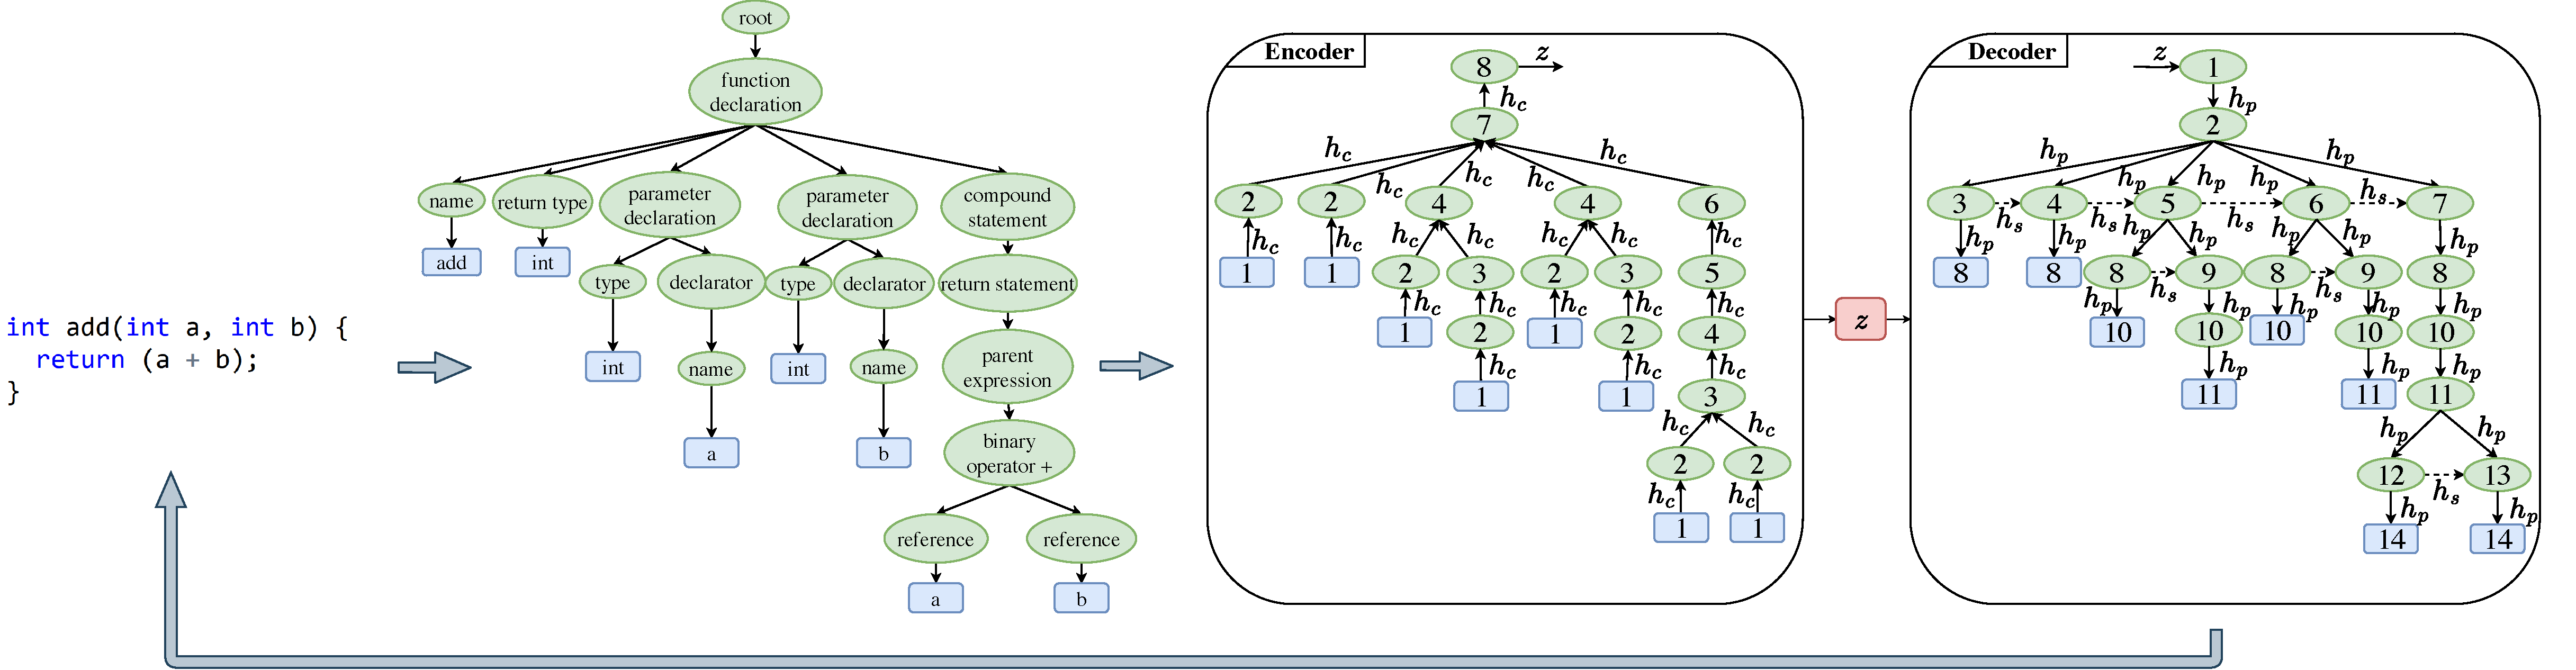
\includegraphics[width=\linewidth]{tree2treeLSTM2.pdf}
    \caption[Tree2Tree model high-level overview]{Tree to tree autoencoder overview. \textbf{First Fig.}: The piece of code considered. \textbf{Second Fig.}: The piece of code parsed to an AST tree format. \textbf{Third Fig.}: The order in which the encoder module encodes the tree structure bottom-up. Here, $h_c$ indicates the hidden state that travels from a child to a parent. \textbf{Fourth Fig.}: The order in which the decoder module decodes the tree structure top-down. Here, $h_p$ indicates the hidden state that travels from a parent to a child, and $h_s$ indicates the hidden state that travels from a node to its successor sibling.}
    \label{fig:tree2treeVAE}
\end{figure}

\newpage
\section{Evaluation}
\label{sec:tree2tree-eval}

\subsection{Dataset}
\label{sec:tree2tree-dataset}
We train and evaluate our model on a dataset of programs from code competition websites: programs from these platforms exhibit a few qualities that are suitable for program synthesis. The programs are tested and known to be syntactically correct, compile-able and standalone, i.e. they do not depend on any code that is not built into the programming language. 

The dataset consists of almost two million C++ programs across 148 competitions divided over 904 problems. 
Hence, on average, each contest contains around six problems to solve with about 2,000 programs for each problem, see table \ref{tab:statistics_contests_problems} for more statistics. 

\begin{table}
\centering
% A table with adjusted row and column spacings
% \setlength sets the horizontal (column) spacing
% \arraystretch sets the vertical (row) spacing
\begingroup
\setlength{\tabcolsep}{8pt} % Default value: 6pt
\renewcommand{\arraystretch}{1.6} % Default value: 1
\begin{tabular}{c|ccccc}
  & \textbf{Total} & \textbf{Mean \#} & \textbf{Median \#} & \textbf{Min \#} & \textbf{Max \#} \\ \hline
\textbf{Contests} & 148 & 13,277 & 13,383 & 36 & 51,460 \\
\textbf{Problems} & 904 & 2174 & 898 & 1 & 19,790 \\
\end{tabular}
\caption[Data set statistics]{Data set statistics in terms of number of contests, problems and statistics on number of programs within contests and problems.}
\label{tab:statistics_contests_problems}
\endgroup
\end{table}

We also measure program size in terms of number of tokens: keywords, identifiers, operators, or special symbols (e.g., a semicolon or brace): figure \ref{fig:program_sizes}
 depicts the size distribution. 
 The longest program in the dataset is 27882 tokens.

\begin{figure}
    \centering
    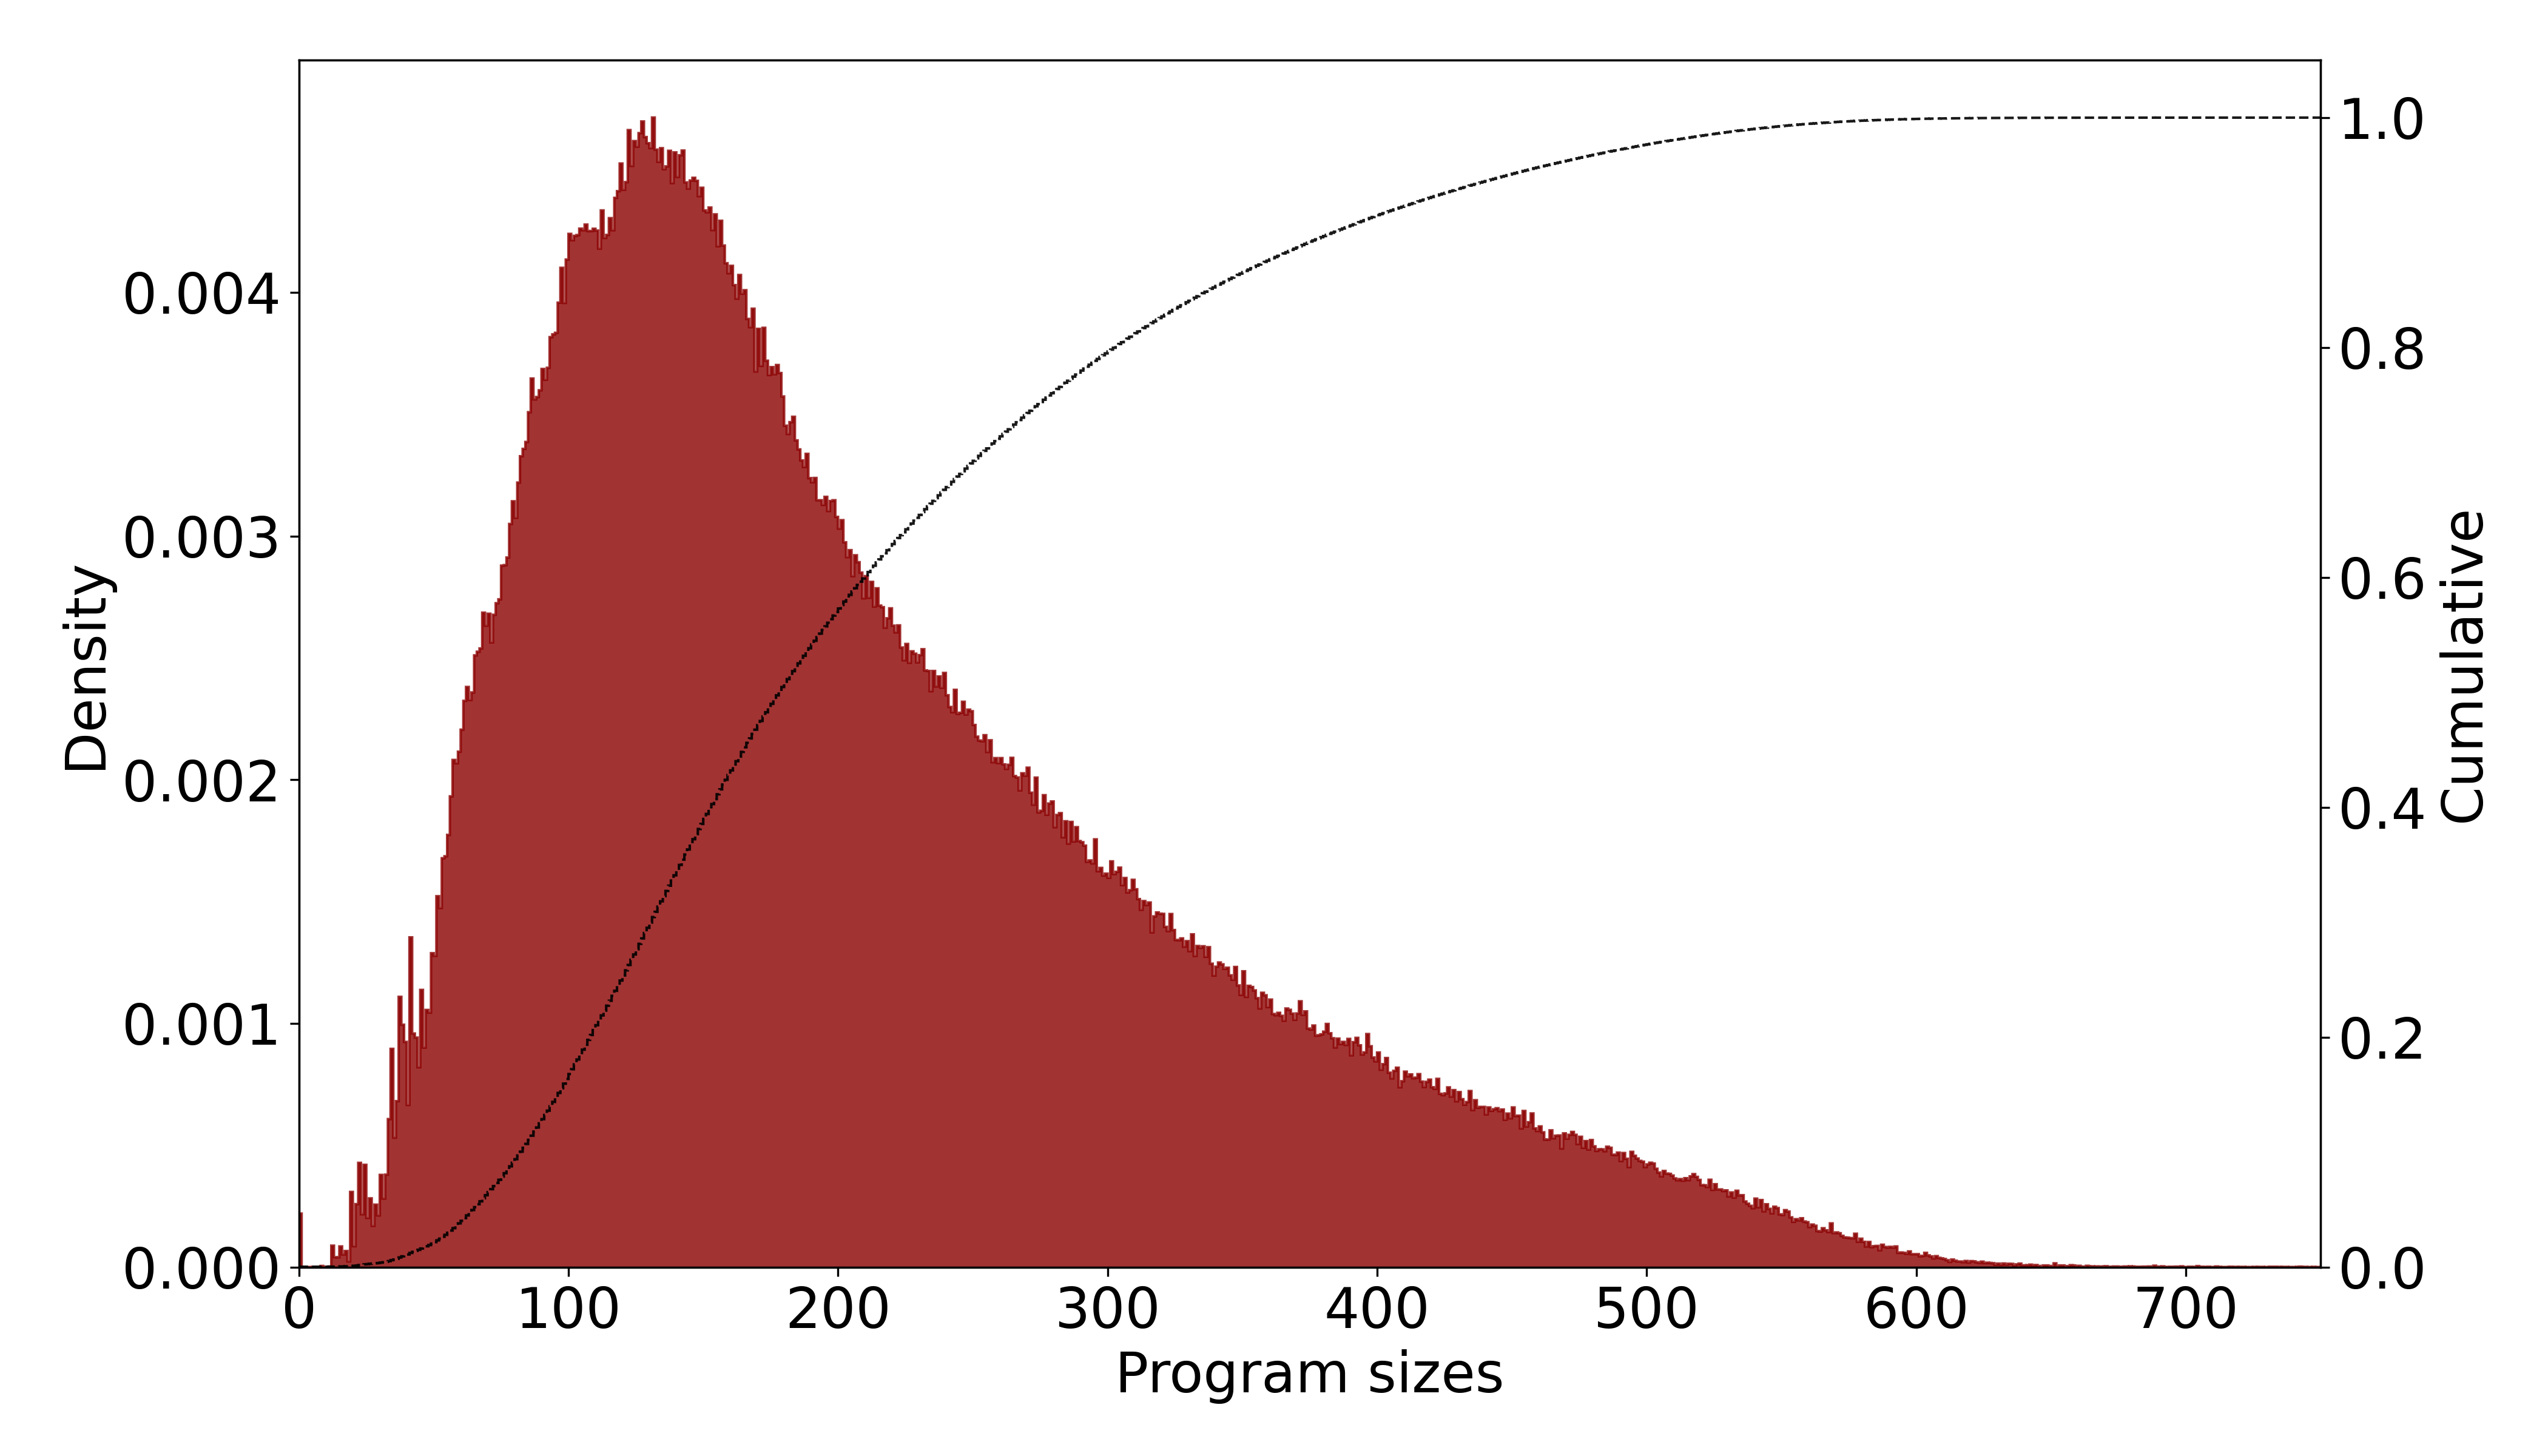
\includegraphics[width=\linewidth]{images/program_sizes.png}
    \caption[Distribution of program sizes]{Distribution of program sizes in terms of number of tokens. The black line indicates the cumulative density.}
    \label{fig:program_sizes}
\end{figure}

The programs in the dataset generally contain a main function, standard input and output stream elements, computation and memory optimizations, and possibly other elements such as helper functions/classes. Due to this general structure, the programs tend to overlap in their content, in contrast to, for example, natural language sentences. 
Due to the limitations on performance imposed by code contests, these programs contain an unusually high amount of low-level optimizations, such as \verb|sync_with_stdio(false); cin.tie(nullptr);| for faster input and output \cite{FastInputOutput}.

\subsection{Pre-processing}
\label{sec:preprocessing}

Very long programs are challenging for our experiments both as statistical outliers and due to the high computational cost of processing them. We thus exclude all programs that exceed 750 tree nodes, approximately 5\% of the dataset.

Comments, imports and macros are removed from the programs.
Comments can be removed safely without altering the program's execution, all imports present in the dataset are collected in a separate file and added to every reconstructed program, and macros are expanded in-place.
We use CLANG C++ compiler to expand macros, as well as parse the programs as Abstract Syntax Trees (ASTs) for training.

\subsection{Baseline}

Our baseline model is a maximally simple sequence to sequence (Seq2Seq) autoencoder based on a single layer Gated Recurrent Unit \cite{chung2014empirical} architecture. Similar to Tree2Tree, we employ methods to mitigate KL-vanishing, namely, cyclic KL annealing \cite{fu2019cyclical} and word dropout \cite{bowman2015generating}.

\subsection{Training parameters}

\begin{table}
\centering
\begin{tabular}{r|c|c}
\textbf{Hyper parameter} & \textbf{Seq2Seq} &      \textbf{Tree2Tree} \\
\hline
                   Epochs &                10 &                      10 \\
               Batch size &                32 &                      32 \\
            Learning rate &              1e-4 &                    1e-3 \\
        Recurrent dropout &               0.2 &                     0.2 \\
      Embedding dimension &                 50&                      50 \\
 Embedding initialization &            random &  Glove wiki gigaword 50 \\
                Optimizer &              Adam &                    Adam \\
  Early stopping patience &                 3 &                       3 \\
\end{tabular}

\caption{Training hyperparameters for baseline and Tree2Tree models}
\label{tab:params}
\end{table}

Table \ref{tab:params} lists the hyperparameters selected for training the baseline and the proposed model.
Note that the only difference is the learning rate (set experimentally) and pre-trained embeddings.
Since we use word vectors designed for English\footnote{The only token embedding effort for C++ we are aware of \cite{harerAutomatedSoftwareVulnerability2018} does not publish the coefficients}, not C++, we do not expect their use to be beneficial for embedding leaf nodes (tokens that occur in the code directly, i.e. \verb|+|).
However, non-leaf nodes of the AST have interpretable labels such as "function declaration", so we expect GLoVe \cite{pennington2014glove} embeddings in the Tree2Tree model to be meaningful.

\newpage
\section{Results}
\label{sec:results}

\subsection{Quantitative assessment}

\paragraph{Reconstruction results}\label{sec:recon-results}
First, we look at how accurately the autoencoders can reconstruct programs. We use a separate test split containing around 60000 samples of our data set to evaluate this and use these samples as input for the autoencoders. 


We compute ground truth similarity scores for both models on the original representation of the source code to obtain comparable results, i.e., we do not use the tree representation.
The Tree2Tree model thus has an extra step to use the data parser to transform the tree representation back to source code. This extra step is disadvantageous for the Tree2Tree model as it may introduce errors due to imperfections in the parsing process. 
We choose BLEU \cite{papineni2002bleu} as the similarity metric to maintain consistency with recent code generation literature \cite[table I]{evtikhievOutBLEUHow2023}.
The BLEU scores are then computed on each token in a program: keywords, identifiers, operators, and special symbols such as semicolons or braces. 
We report on the cumulative BLEU-1 through BLEU-4 scores to indicate the overlap between original and reconstructed programs, as well as present the percentage of reconstructed programs that compile to indicate how well the models have learned the programming language's syntax. We experiment with different combinations of latent sizes $|\latent|$ and hidden RNN dimensions $|\hidden|$:  ($|\latent|$:10,  $|\hidden|$:50), ($|\latent|$:50, $|\hidden|$:100), ($|\latent|$:100, $|\hidden|$:200), ($|\latent|$:150, $|\hidden|$:300), ($|\latent|$:300, $|\hidden|$:500), ($|\latent|$:500, $|\hidden|$:800), ($|\latent|$:800, $|\hidden|$:1200).


We use greedy decoding in reconstruction experiments (\ref{tab:rec_results}) to maximize accuracy. In contrast, sampling is used in generation tasks where diversity of candidates can be helpful.

\begin{table}
\centering
% A table with adjusted row and column spacings
% \setlength sets the horizontal (column) spacing
% \arraystretch sets the vertical (row) spacing
\begingroup
\setlength{\tabcolsep}{3pt} % Default value: 6pt
\renewcommand{\arraystretch}{1.4} % Default value: 1
\begin{tabular}{cccccccc}
 & \textbf{Latent} & \textbf{BLEU-1} & \textbf{BLEU-2} & \textbf{BLEU-3} & \textbf{BLEU-4} & \textbf{Compiles}\\ \hline
\multirow{7}{*}{Seq}    &   10   &  0.037   &    0.024     &     0.017     &    0.013       &    0.000\%   \\
                            &   50   &      0.085    &      0.061         &         0.047      &    0.037       &       42.467\%      \\
                            &   100   &  0.295   &      0.225     &     0.176      &    0.141       &   65.808\%               \\
                            &   150   &     0.278  & 0.211          & 0.165          & 0.131          &  66.971\%              \\
                            &   300   & 0.346                     &  0.262                        &     0.203                     &     0.161                     & 60.651\% \\   
                            &   500   &  0.421                   &      0.332                    &         0.263                 &      0.211                    &  90.329\% \\
                            &   800   &  0.429                   &      0.329                    &         0.253                 &      0.195                    &  \textbf{91.784\%} \\\hline
\multirow{7}{*}{Tree}  &   10   &  0.445  &    0.339     &     0.260     &     0.202      &   28.375\%    \\
                        &   50   &     0.417    &      0.317    &       0.242    & 0.189  &  23.256\% \\
                            &   100   &     0.423      &      0.323     &     0.251      &  0.200 &      30.429\%     \\
                            &   150   & \textbf{0.486} &     \textbf{0.382}    &  \textbf{0.302}     &      \textbf{0.243}    &   35.419\%           \\
                            &   300   &   0.457                 &     0.342                &      0.260                &     0.202                   & 35.054\% \\   
                            &   500   &     0.398                &      0.301             & 0.230      &             0.178             &            36.022\%      \\
                             &   800   &     0.258                &      0.182             & 0.131      &             0.096             &     2.358\%      \\
\end{tabular}
\endgroup
\caption{Reconstruction results.}
\label{tab:rec_results}
\end{table}

The results listed in table \ref{tab:rec_results} show the superiority of the Tree2Tree model in terms of reconstruction capability (BLEU scores), especially for smaller latent sizes. The reconstruction scores of the Tree2Tree model of latent size 150 outperform all the Seq2Seq models up to latent size 800. In contrast, the Seq2Seq models show to perform much better at constructing compile-able programs, which improves with the model's size, to nearly 100\%. This is a surprising result, which is investigated in more detail in section \ref{sec:tree2tree-eval}.

 


An interesting result is that the performance of the models does not necessarily increase with the size of the model. Especially for the Tree2Tree models, we see that after latent size 150, the models' performance decreases. In general, one would expect that the model would perform better with an increase in latent size, allowing more information flow between the encoder and decoder. We hypothesize that, because not only the latent size increases but also the number of hidden units in the autoregressive models, the models experience KL vanishing. Due to the increasing hidden units, the autoregressive models become stronger and may depend more on their predictions, ignoring information from the latent vector. In turn, the reconstruction performance vastly decreases. Confirmation of this hypothesis is left as a venue for future work.



Next, we evaluate the effect of different input sizes on the performance of both models. Due to the tree-structured representation used Tree2Tree, the size of the sequences that the RNNs process scales proportionally to the width and depth of the tree. The Seq2Seq model, on the other hand, processes sequences left to right, hence the number of computations of the RNNs scales directly with the sequence length. 



To evaluate the performance on different sized inputs, we split the test data set into three subsets. A small, medium and large subset with the following properties:

\begin{itemize}
    \item \textbf{small subset}: maximum of 250 tokens
    \item \textbf{medium subset}: between 251 and 500 tokens
    \item \textbf{large subset}: between 501 and 750 tokens
\end{itemize}

 

We compute the BLEU scores and compilation percentage again using greedy decoding on the smaller subsets for the best performing Seq2Seq and Tree2Tree models, based on the results of table \ref{tab:rec_results}. Here, performance is based on the combination of BLEU-4 and compilation percentage. For Seq2Seq, this is the model with latent size 500. Similarly, for Tree2Tree, this is the model with latent size 150. The results are depicted in table \ref{tab:rec_results_in\prob_sizes}.



%150 latent t2t lr 0.001 large test set (> 500, <= 750): bleu1 0.317, bleu2 0.236, bleu3 0.177, bleu4 0.134, compiles 5.001

%150 latent t2t lr 0.001 medium test set (> 250, <= 500): bleu1 0.468, bleu2 0.364, bleu3 0.284, bleu4 0.225, compiles 21.241


\begin{table}
\centering
% A table with adjusted row and column spacings
% \setlength sets the horizontal (column) spacing
% \arraystretch sets the vertical (row) spacing
\begingroup
\setlength{\tabcolsep}{3pt} % Default value: 6pt
\renewcommand{\arraystretch}{1.4} % Default value: 1
\begin{tabular}{clccccc}
 & \textbf{Input} & \textbf{BLEU-1} & \textbf{BLEU-2} & \textbf{BLEU-3} & \textbf{BLEU-4} & \textbf{Compiles}\\ \hline
\multirow{3}{*}{Seq}    &   small   &   0.513  &    0.403    &      0.321    &  0.258      &  95.334\%     \\
                            &   medium   &  0.306      &    0.244        &      0.192     & 0.153      & 86.812\% \\
                            &   large   &    0.196   &      0.157   &   0.123       &   0.096       &  87.971\% \\ \hline
\multirow{3}{*}{Tree}  &   small   &   0.633  &    0.516     &     0.424     &     0.355      &  59.022\%                \\
                            &   medium   &   0.478  &   0.371        &          0.289 &     0.229   & 21.241\%            \\
                            &   large   &  0.324 &      0.242  & 0.181    &    0.138     &    5.001\%         \\ 
\end{tabular}
\endgroup
\caption{Reconstruction results of the best models on different input sizes.}
\label{tab:rec_results_in\prob_sizes}
\end{table}



From table \ref{tab:rec_results_in\prob_sizes} we can glean that both models follow the same trend: the larger the input size, the lower BLEU-scores and compilation percentages. For the Tree2Tree model, the BLEU scores for the medium subset seem to be similar to the BLEU scores on the entire test set, whereas, for the Seq2Seq model, the BLEU scores are much lower on the medium subset. The models seem to be fairly close in terms of performance degradation from small to large program sizes. For example, we can measure performance degradation for the large versus small subset by dividing the BLEU-4 scores on the large set by the BLEU-4 score on the small set. For the Seq2Seq model, we get a score of $0.372$, and for the Tree2Tree model, we get $0.389$. Similarly, we get $0.593$ and $0.645$ for the Seq2Seq and Tree2Tree model for the medium versus small subset. While the performance degrades less with increasing input sizes for the Tree2Tree model, this difference is insignificant. 

An issue with this computation of performance degradation is that it does not correct for boilerplate elements present in most programs, such as a main function with standard input and output streams. 
This causes the BLEU score to consist of two parts:  prediction of the elements that are always present and accurate reconstruction of the original program. 
Therefore, we apply a correction on the BLEU scores to focus on the prediction based on the information in the latent vector. 
We compute corrected scores by feeding the decoder with random latent vectors and computing BLEU scores on the subsets of the test data set. 
Then, we subtract these correction scores from the computed BLEU scores in table \ref{tab:rec_results_in\prob_sizes}, and take 0 if the result of the subtraction is negative. The corrected BLEU scores including the correction scores are in table \ref{tab:corrected_rec_results_in\prob_sizes}.

\begin{table}
\centering
% A table with adjusted row and column spacings
% \setlength sets the horizontal (column) spacing
% \arraystretch sets the vertical (row) spacing
\begingroup
\setlength{\tabcolsep}{3pt} % Default value: 6pt
\renewcommand{\arraystretch}{1.4} % Default value: 1
\resizebox{\linewidth}{!}{%

\begin{tabular}{clccccc}
\textbf{Model}   & \textbf{Input size} & \textbf{BLEU-1} & \textbf{BLEU-2} & \textbf{BLEU-3} & \textbf{BLEU-4} \\ \hline
\multirow{3}{*}{Seq2Seq}    &   small   &   0.072 (0.441)  &    0.077 (0.326)    &  0.075    (0.246)    &  0.070 (0.188)     \\
                            &   medium   & 0.006 (0.300)      &  0.018  (0.226)        &    0.021  (0.171)     & 0.023 (0.130)    \\
                            &   large   &   0.000 (0.213)   &  0.000    (0.166)   & 0.000  (0.128)       &  0.000 (0.099)   \\ \hline
\multirow{3}{*}{Tree2Tree}  &   small   &  0.200 (0.433)  &  0.220  (0.296)     &  0.223   (0.201)     &    0.218 (0.137)        \\
                            &   medium   &  0.148 (0.330)  &  0.147 (0.224)        & 0.146 (0.150) &    0.128 (0.101)        \\
                            &   large   &  0.102 (0.222) &    0.090  (0.152)  &  0.079 (0.102)     &  0.070  (0.068)      &   \\
\end{tabular}%
}
\endgroup

\caption{Corrected BLEU scores of reconstructed results of the best models on different input sizes. (correction scores in parentheses)}
\label{tab:corrected_rec_results_in\prob_sizes}
\end{table}



Table \ref{tab:corrected_rec_results_in\prob_sizes} indicates a large difference in performance degradation between the Seq2Seq model and the Tree2Tree model. A noticeable result is that the corrected BLEU scores for large programs predicted by the Seq2Seq model are 0. Hence, the Seq2Seq model extracts no information from the latent vector at all for large programs. Similarly, for medium-sized programs, little information is transferred between the encoder and decoder. We can again compute the performance degradation scores for the Seq2Seq model, which are $0.280$ and $0.00$ for the medium versus small and large versus small subsets, respectively, on the corrected BLEU-4.



In contrast, the performance degradation is much smaller for the Tree2Tree model:  $0.587$ and $0.321$ for the medium versus small and large versus small subsets, respectively, on the corrected BLEU-4. Hence, the structural nature of the Tree2Tree model scales better to large input sequences than the Seq2Seq model in terms of reconstruction scores, even with a much smaller latent size. 



An interesting observation is that the latent vector conveys relatively little information in terms of BLEU scores. The correction scores make up a large part of the total BLEU scores as presented in table \ref{tab:rec_results_in\prob_sizes}. Hence, the BLEU scores are largely determined by the models' general knowledge of how C++ programs are built up and not the specific content.

\paragraph{Generative results}
\label{results:gen}
To see how well autoencoders can generate reasonable samples from any point in latent space that conform to the C++ syntax, we sample 1000 random latent vectors from the prior distribution $\normaldistr(0, I)$ and input these vectors to the decoder networks. Then, we compute the percentage of generated programs that compiles and is thus also syntactically correct.



We employ two decoding strategies to test the generative capabilities of the models: greedy decoding and sampling. The sampling strategy we apply is a combination of top-$k$, nucleus, and temperature sampling \cite{holtzman2019curious}. 
We first use temperature sampling to scale the logits to control the shape of the probability distribution. Then we discard all but the top $k$ samples, after which we filter tokens on their cumulative probability using nucleus sampling (top-$p$). Lastly, we sample a token from the resulting distribution. The selected sampling hyperparameters for this experiment are: $k=40$, $p=0.9$, $temperature=0.7$. The results are displayed in table \ref{tab:gen_results}.

\begin{table}
\centering
% A table with adjusted row and column spacings
% \setlength sets the horizontal (column) spacing
% \arraystretch sets the vertical (row) spacing
\begingroup
\setlength{\tabcolsep}{3pt} % Default value: 6pt
\renewcommand{\arraystretch}{1.4} % Default value: 1
\begin{tabular}{cccc}
\textbf{Model}   & \textbf{Latent size} & \textbf{Greedy search} & \textbf{Sampling} \\ \hline
\multirow{5}{*}{Seq2Seq}    &   10   &  0.0\%   & 0.9\%  \\
                            &   50   &   38.5\%    &  2.9\%   \\
                            &   100   &   62.1\%   &  21.3\%     \\
                            &   150   &   58.0\%  &     23.5\%        \\
                            &   300   &  60.6\%  &  36.8\%   \\   
                            &   500   &  67.5\% & 37.8\% \\
                            &   800   & 78.2\%  & 39.6\% \\\hline
\multirow{5}{*}{Tree2Tree}  &   10   &   29.6\%   & 20.2\% \\
                            &   50    & 22.6\%   &  17.7\%    \\
                            &   100    & 30.3\%  &       22.1\%      \\
                            &   150  &  26.9\%  &   18.8\%     \\
                            &   300  & 23.4\%  & 12.8\%    \\   
                            &   500 & 25.6\%  & 14.4\%\\
                            &   800   &  4.1\% & 6.7\% \\
\end{tabular}
\endgroup
\caption{Generative results compilation percentage.}
\label{tab:gen_results}
\end{table}




The results from table \ref{tab:gen_results} show similar trends as section \ref{sec:recon-results}. 
The general trend is: the larger the model (in terms of latent size and hidden units), the higher the compilation percentage. 
We can also see the trade-off between a higher compilation ratio achieved with greedy search and a more diverse output with sampling that can be useful for exploring similar programs in a vicinity of the latent space.

\newpage
\subsection{Qualitative assessment}

\begin{figure*}
  \centering
  \includegraphics[width=\textwidth,height=\textheight,keepaspectratio]{images/reconstruction_examples2.pdf}
  \caption{Examples of reconstructed programs}
  \label{fig:rec_examples}
\end{figure*}

In addition to quantitative results, we compare actual examples of reconstructions generated by both models with each other and the original program, see figure \ref{fig:rec_examples}. 

A noticeable difference between the original programs and the programs produced by the models is the removal of the definitions (macros). 
As discussed in \ref{sec:preprocessing}, expanding macros is part of the data pre-processing stage. However, if the macros are not used in the program, they will not affect the source code and are removed. The original program in the top row contains many macros that are not used in the code fragment. From these examples, we can hypothesize that code competition participants tend to use a template file with a list of predefined macros to speed up the programming task.



Overall, figure \ref{fig:rec_examples} shows that the programs generated by the Tree2Tree model are much more similar to the original programs than the programs generated by the Seq2Seq model. For the top row, the Tree2Tree model programs' is content is the same as the original program (except for an end line that is inserted into the output stream.) In contrast, the program of the Seq2Seq model shares some similarities to the original, but the functionality is vastly different. A similar story holds for the middle and bottom rows, where the programs of the Tree2Tree model are not as close to the original program as in the top row. However, they are still much closer than the programs generated by the Seq2Seq model. 



The reconstruction examples show how the models have learned the C++ syntax. Both models always return 0 at the end of the main function in the examples, even if this is not present in the original program. Furthermore, due to the extracted AST from the compiler, the Tree2Tree model has learned to initialize certain types such as maps or vectors. The C++ compiler does not require this and also is not present in the original programs. Additionally, the Tree2Tree model seems to have learned that certain elements may be interchanged without changing the functionality. For example, use 0 instead of NULL when decoupling the standard input stream in the top row example. 



Another interesting observation in figure \ref{fig:rec_examples} is that the Seq2Seq has produced the same reconstruction for both the top and bottom row. The Seq2Seq maps the same program to multiple latent vectors, indicating some form of KL vanishing where the decoder partly ignores the latent vector. Mapping the same programs to multiple latent vectors limits the reconstructions capabilities, as multiple original programs will be mapped to the same reconstructed program. This mapping may also explain the high compilation percentage for the Seq2Seq model, as it may simply remember a small population of programs that is compile-able and overlaps for a large part with the original programs. 



For the Tree2Tree model, the reconstructions examples show that a problematic aspect of reconstruction is predicting the literals such as strings and numbers correctly. Furthermore, the model also has some issues with predicting references to identifiers correctly or the correct types. In contrast, the model performs well at reconstructing the general structure of programs, such as where to place functions, for-loops, and if-statements. An example of this is shown in the bottom row of figure \ref{fig:rec_examples}, where the structure of quite a long program is reconstructed accurately for the most part. 

\begin{figure}
    \centering
    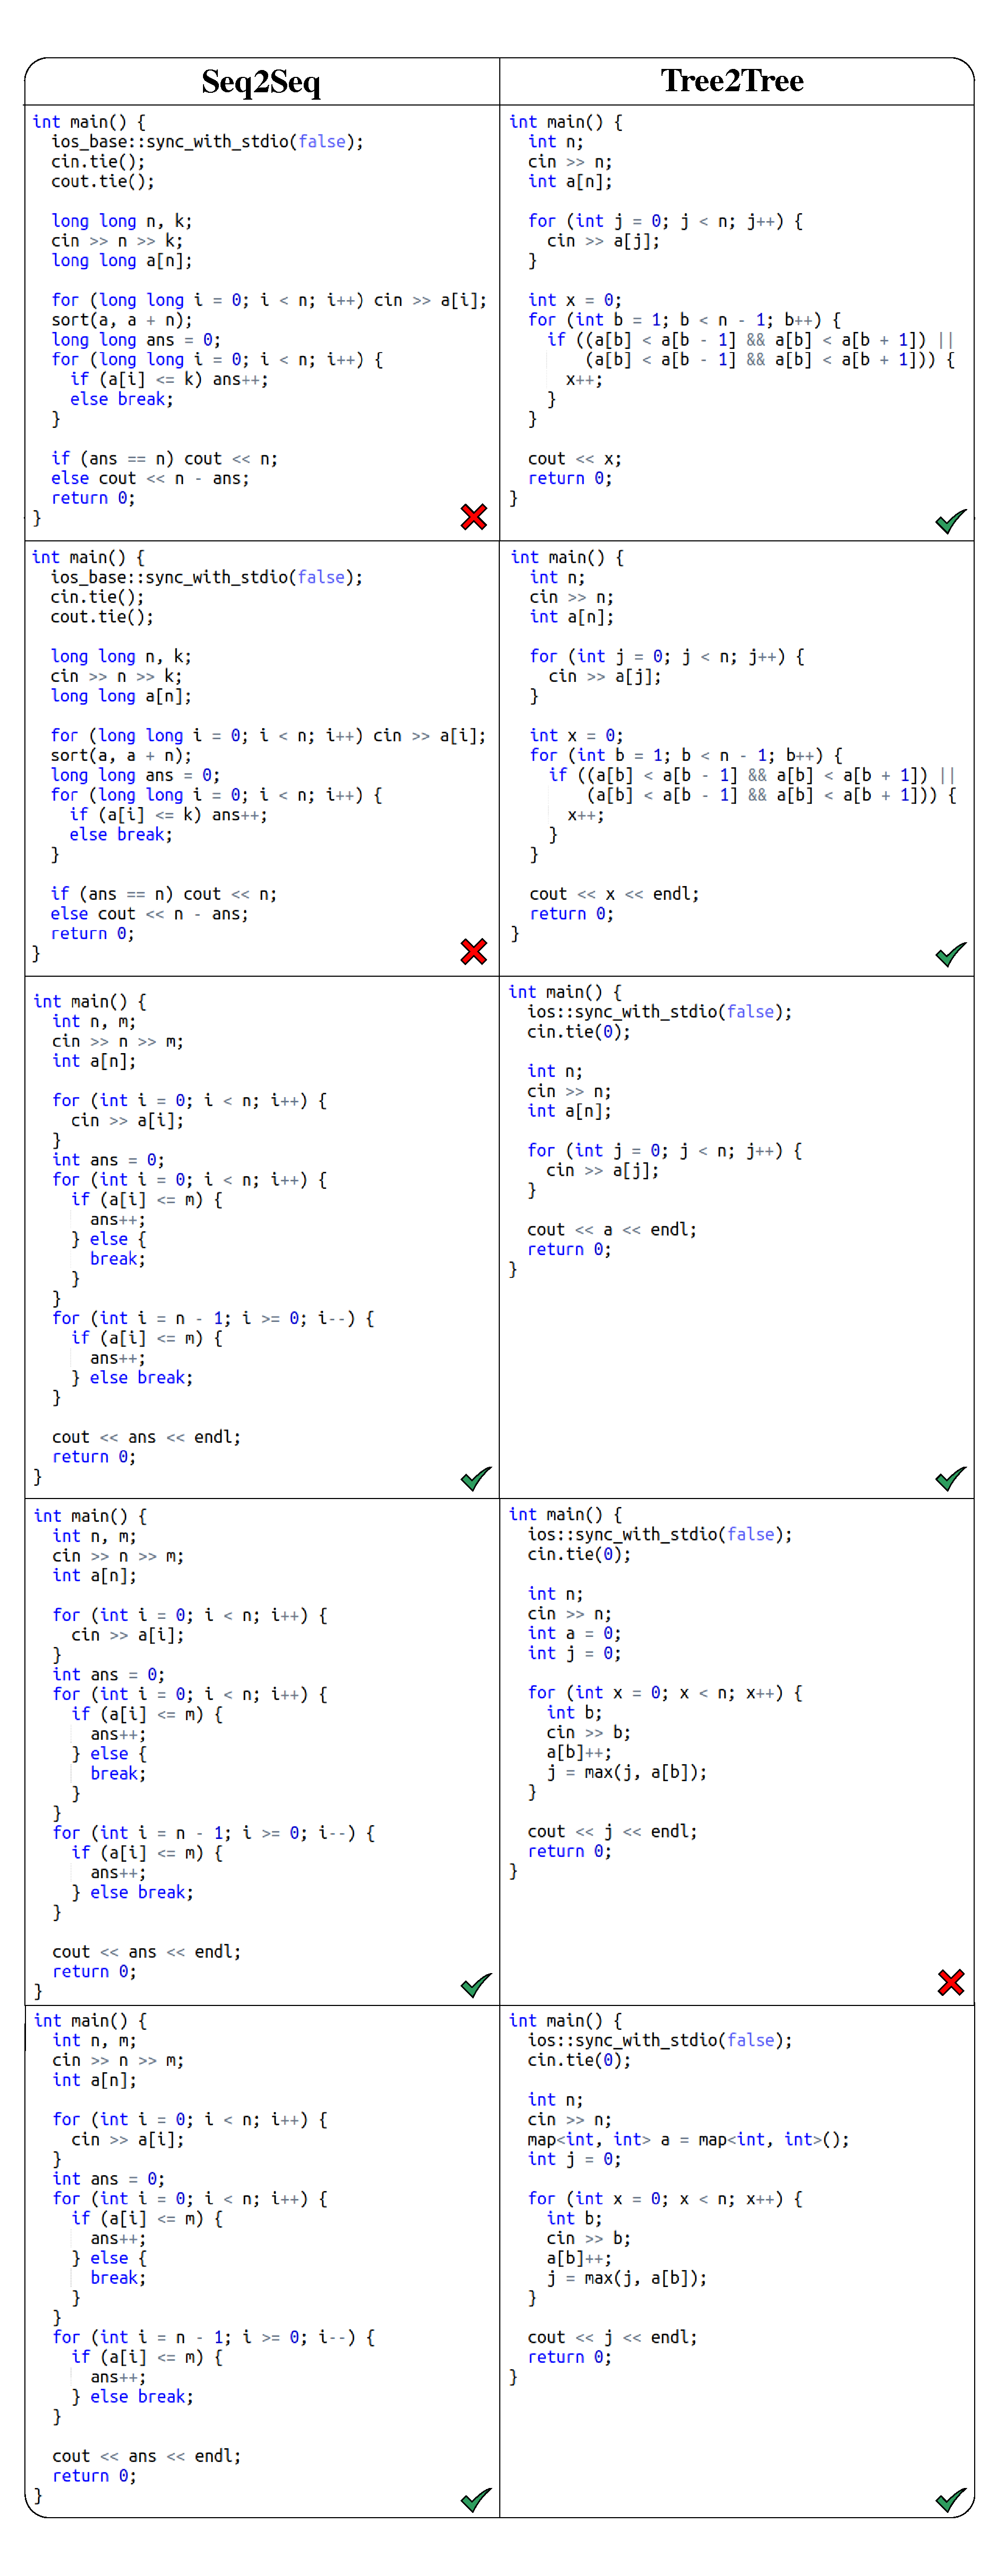
\includegraphics[width=\textwidth,height=\textheight,keepaspectratio]{images/Interpolations.pdf}
    \caption{Examples of interpolated programs. The check-marks/crosses in the bottom-right indicate whether the programs compile.}
    \label{fig:interpolation_examples}
\end{figure}

Secondly, we can explore interpolations between two data points in latent space by randomly selecting two samples from our test set and averaging them in the latent space, see figure \ref{fig:interpolation_examples}. The interpolations run from top to bottom, where the top and bottom programs represent a data point, and the three programs in between represent the interpolations. The bottom-right corner contains either a cross or a checkmark indicating whether the program is compile-able.


The Seq2Seq model displays similar behavior as with the reconstructions, multiple latent vectors map to the same program. The top two programs are the same, and the bottom three programs are the same. The model does not generate any new programs from the interpolated vectors. This result again indicates that the Seq2Seq decoder has learned to deprioritize the latent state and output programs independent of its input. 

The Tree2Tree model makes minor alterations to the programs each interpolation step, transforming it closer to the other data point. This slow shift from one program to another shows how in the latent space of the Tree2Tree model, similar points in latent space also map to similar programs. This is a valuable property for GP, as this allows for a directed search over the latent space. Furthermore, a large part of the interpolations is compile-able, which is also a valuable property for searching over the latent space of new programs. Only the fourth program down is not compile-able due to the model treating the identifier $a$ as an array while it is declared an integer. This result is interesting, as in both the data points, the identifier $a$ is not declared an integer. In conclusion, the Tree2Tree model has a structured latent space, however, it is not guaranteed that all interpolations between two compile-able programs also result in compile-able programs.
\newpage
\section{Conclusion}

Our results indicate that Tree Variational Autoencoders have a significant advantage over sequence-to-sequence models in low-dimensional latent spaces, achieving both a higher compilation rate and a higher reconstruction quality.
In higher-dimensional latent spaces seq2seq programs offer a higher compilation rate, but corrected BLEU scores indicate that this benefit is often achieved by sacrificing reconstruction quality, even to the point of ignoring the input completely.

Overall, our findings support the initial hypothesis that structured autoencoder models are better suited for program synthesis than sequence-to-sequence alternatives.
We believe this result to be a significant step towards an autoencoder-based foundation model for genetic programming and genetic improvement of software.